\section{Ground station networks}

There are a lot of unknowns in this area. We don't know which network will be used, who will be participating or what kind of radio equipment participants will have. 

Some different possible networks are simulated using the same constraints as at Gløshaugen.

\begin{figure}
\begin{subfigure}{.5\textwidth}
	\centering
	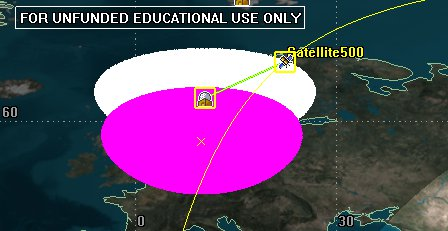
\includegraphics[width=\textwidth]{Figures/range_ntnu_aalborg}
	\label{fig:range_ntnu_aalborg}
\end{subfigure}
\begin{subfigure}{.5\textwidth}
	\centering
	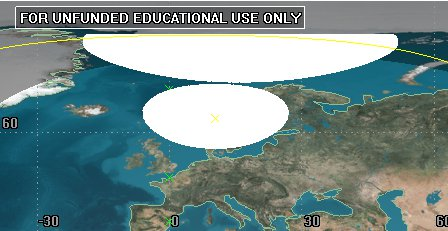
\includegraphics[width=\textwidth]{Figures/range_ntnu_svalbard}
	\label{fig:range_ntnu_unis}
\end{subfigure}
\begin{subfigure}{.5\textwidth}
	\centering
	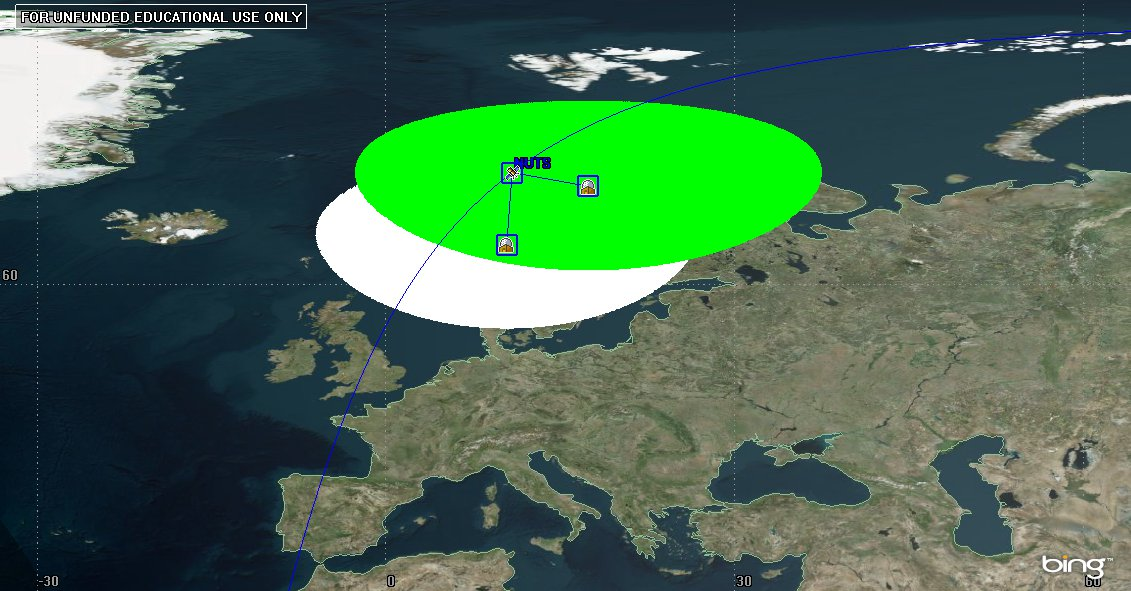
\includegraphics[width=\textwidth]{Figures/range_ntnu_narvik}
	\label{fig:range_ntnu_narvik}
\end{subfigure}
\begin{subfigure}{.5\textwidth}
	\centering
	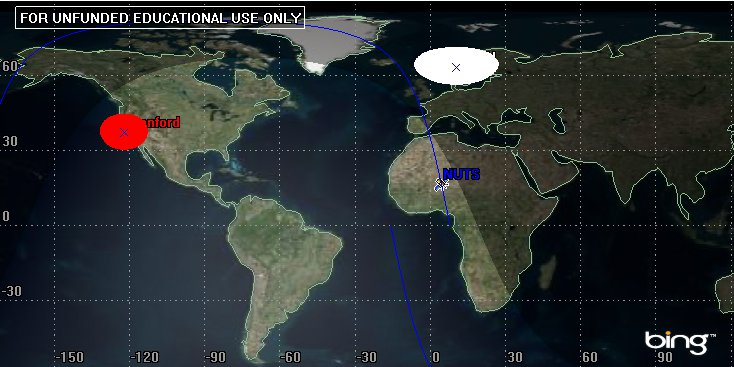
\includegraphics[width=\textwidth]{Figures/range_ntnu_stanford}
	\label{fig:range_ntnu_narvik}
\end{subfigure}
\caption{Some possible ground networks}
\label{fig:ground_networks}
\end{figure}

The results are summarised in Table \ref{tab:networks}.

\begin{table}
	\begin{center}
	\begin{tabular}{l | c c}
  	Other locations & Time & Improvement \\
	\hline \hline
	Aalborg & 790s &  50\% \\
	\hline
	Longyearbyen & 1900s & 260\% \\
	\hline
	Narvik & 900s & 73\%  \\
	\hline
	Stanford & 800s & 54\% 
	\end{tabular}
	\end{center}
	\caption{Some data}
	\label{tab:networks}
\end{table}